%%mark = star, diamond, square, otimes
%\documentclass{article}
%\usepackage{pgfplots}
%\usepackage[justification=centering]{caption}
%\pgfplotsset{compat=newest}
%\begin{document}
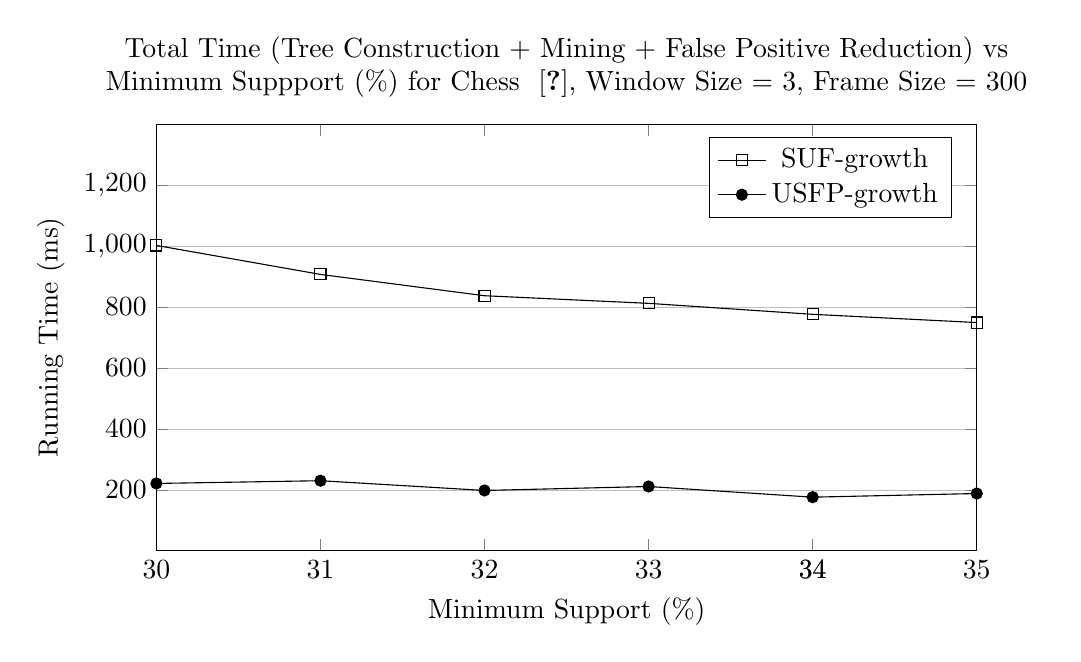
\begin{tikzpicture}
\begin{axis}[
	title={\parbox{\linewidth}{\centering Total Time (Tree Construction + Mining + False Positive Reduction) vs Minimum Suppport (\%) for Chess ~\cite{dataset}, Window Size = 3, Frame Size = 300}},
	width=12cm,
	height=7cm,
    xlabel={Minimum Support (\%) },
    ylabel={Running Time (ms)},
    xmin=30, xmax=35,
    ymin=0, ymax=1400,
    xtick={30,31,32,33,34,34,35},
    ytick={200,400,600,800,1000,1200},
    legend pos=north east,
    ymajorgrids=true,
    grid style={line width=.2pt,draw=gray!50},
]
 
\addplot[
    solid, every mark/.append style={solid, fill=gray}, mark=square
    ]
    coordinates {
			(30,1002)
			(31,907)
			(32,837)
			(33,812)
			(34,776)
			(35,749)
};
    \addlegendentry{SUF-growth}
\addplot[
    solid, every mark/.append style={solid, fill=black}, mark=*
    ]
    coordinates {
			(30,221)
			(31,230)
			(32,198)
			(33,211)
			(34,176)
			(35,188)

};
    \addlegendentry{USFP-growth}
 
\end{axis}
\end{tikzpicture}
%\end{document}